ProtoDUNE is a surface detector that does not have any shielding or veto against the incoming atmospheric flux. This requires a trigger configuration that can exclude the constant stream of cosmic rays while still capturing as many relevant events as possible. %\textcolor{red}{However, several trigger emulations using recorded PD-HD data have shown that the high trigger rates caused by exposure to external background represent a significant challenge, limiting the practical feasibility of multiple trigger algorithms}.

The SPS beam spill lasts 4.8 seconds, which is relatively long for continuous data collection during this time. Furthermore, because the data collection for the neutrino search at the ProtoDUNE detector was parasitic, a single trigger algorithm developed by the DUNE-DAQ group became the only viable solution. This algorithm, known as the \href{https://github.com/DUNE-DAQ/triggeralgs/blob/develop/include/triggeralgs/ADCSimpleWindow/TAMakerADCSimpleWindowAlgorithm.hpp}{ADC Simple Window} algorithm, was modified based on the topology of neutrino interactions within the detector, as studied through neutrino Monte Carlo simulations.

In summary, the ADC Simple Window trigger algorithm consists of two configurable parameters: the time window duration, fixed to 0.32 ms as counseled by the DAQ group, and the ADC threshold. This algorithm works by recording Trigger Primitives (TPs) \cite{abud2023trigger}, which are simplified hits from one readout plane of a single APA frame, until the difference in time between the oldest TP and the most recent TP exceeds the time window length. When the time window is exceeded, the algorithm checks if the sum of ADC charge from all the TPs in the current window is greater than the threshold. If it is, the event gets recorded by merging data from all readout planes and extending the trigger window both before and after the threshold is met. If the threshold is not met, the algorithm adjusts the window to include the next TP, whilst removing the oldest TPs such that length of the time window remains constant, and checks the condition again. This algorithm is summarized in the flow diagram shown in Figure \ref{fig:adcsw_flowdiagram}.

\begin{figure}[ht]
    \centering
    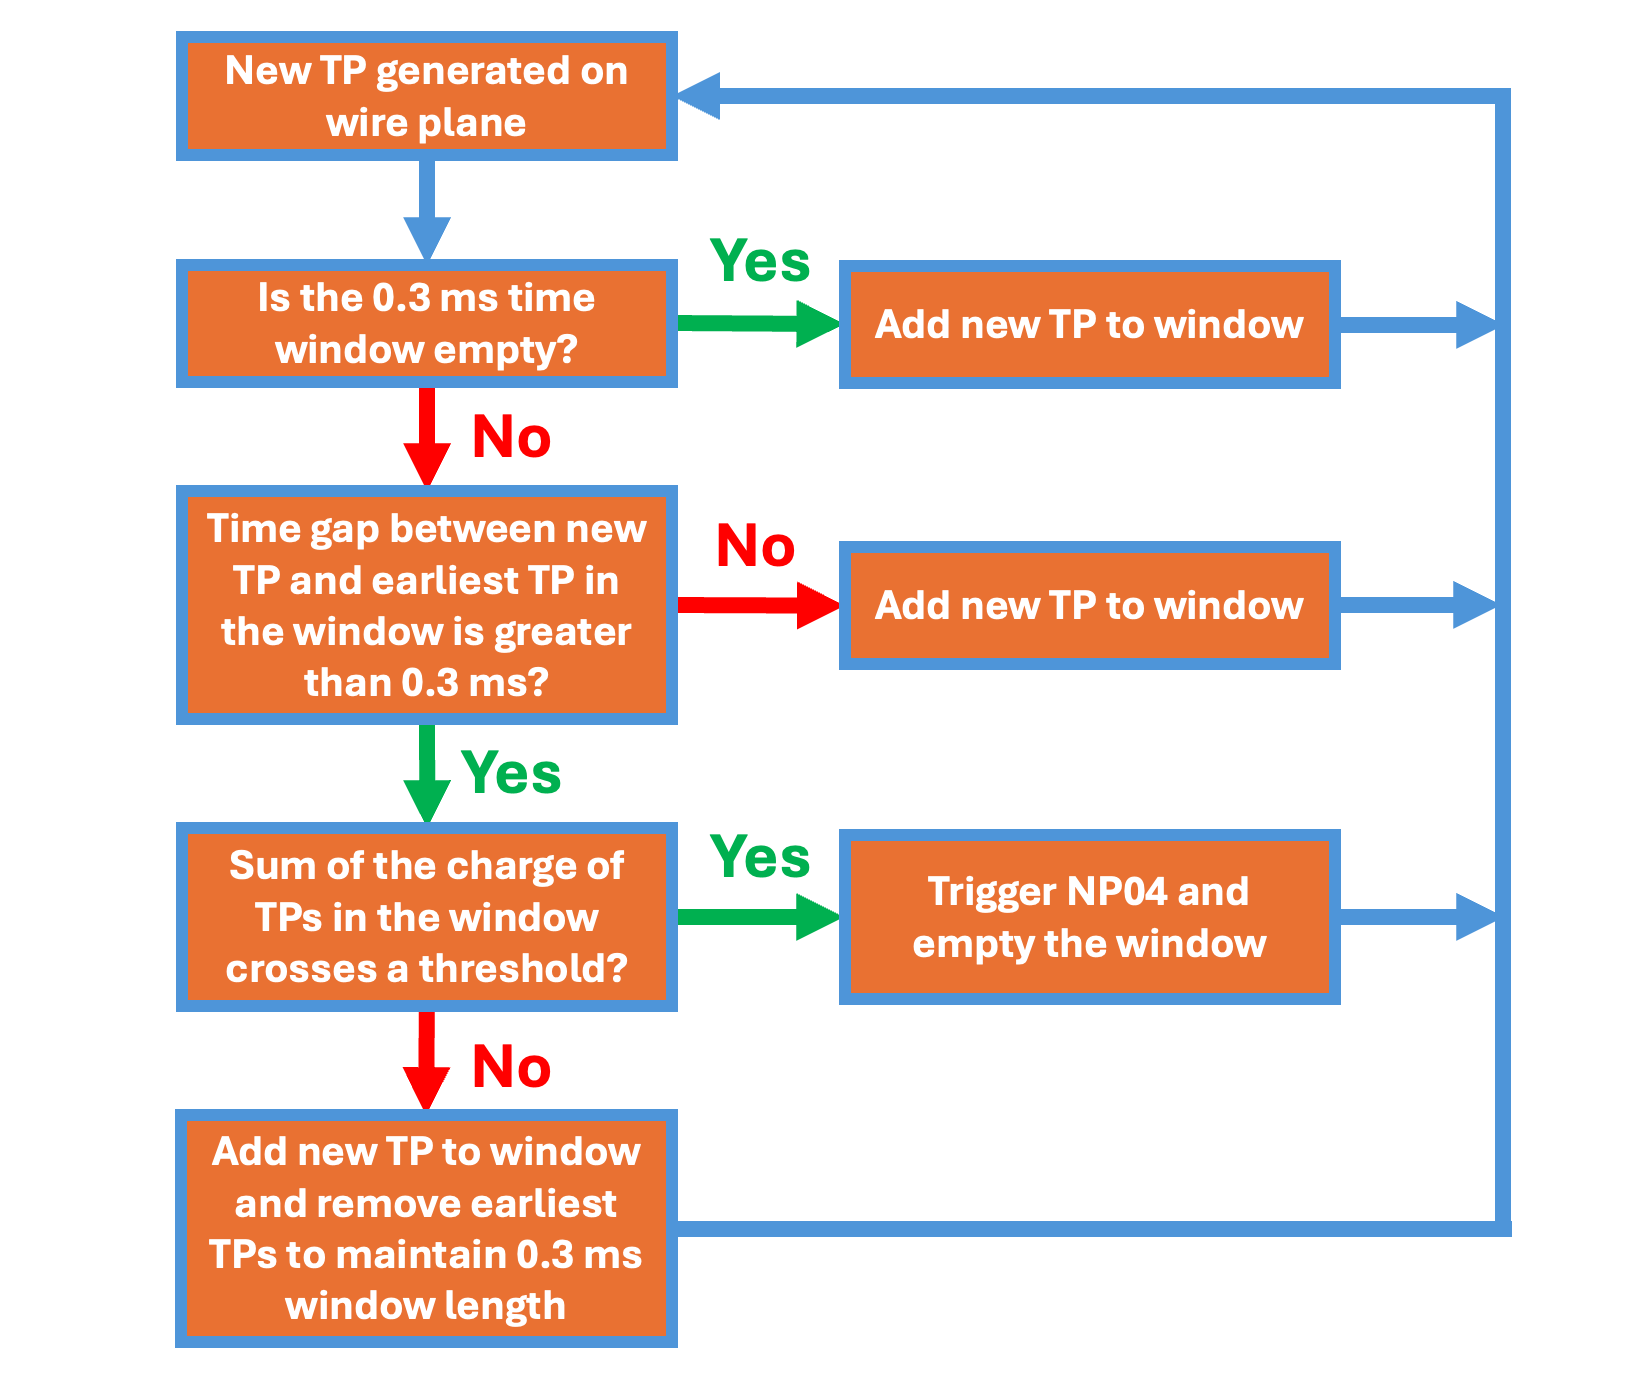
\includegraphics[width=0.8\linewidth]{sections/trigger/plots/ADCSW_flowchart_updated_jan2026.png}
    \caption{A flow diagram summarizing he ADC Simple Window trigger algorithm used to take data at PD-HD. A high charge threshold requirement rejects most cosmic-induced events. The time window refers to an object that contains a list of time-ordered TPs. The length of the time window is set to 0.3~ms, meaning that the difference in time between the earliest and newest TP in the window cannot exceed 0.3~ms.}
    \label{fig:adcsw_flowdiagram}
\end{figure}

The expected charged particle tracks resulting from a neutrino interaction are parallel to the cathode, as explained in section \ref{chap:protodune_det} and illustrated in Figure~\ref{fig:top_view_scheme}. Consequently, events should be confined within a narrow time window. However, to configure the trigger, a Monte Carlo simulation (more in section \ref{chap:montecarlo}) is needed to estimate the trigger efficiency in PD-HD for the incoming neutrino flux. Figure \ref{fig:trigger_performance} shows the simulated trigger efficiency for the cosmic background and the neutrino interactions overlaid with the cosmic rays, for the wNP04 and w133 magnet configurations. At 9 million ADC threshold, the background trigger efficiency is approximately $0.86 \pm 0.18\%$. Then, 99\% of the cosmic-ray events are mitigated, and we kept a stable trigger rate (between 1 and 2 Hz), throughout the data acquisition. Given that the simulated cosmic background readout window has a duration of 4 ms, a maximum of 250 cosmic events would be trigger within a second. Consequently, by multiplying the trigger efficiency, one obtains the expected trigger rate for the background. From the Monte Carlo simulation, a stable trigger is met from 9 million ADCs on. During the campaign, an ADC threshold of 12 million was proved to be the optimal one to ensure a trigger rate ranging between 1 and 2 Hz. Hence, in this study the algorithm employs a time window of 0.32 ms (20000 PDS ticks) and an ADC integral sum threshold of $12 \times 10^6$ ADC, corresponding to $~10-15$ GeV according to the calibration factor extracted in PD-HD from the low energy radiative sources present inside \cite{lavaut2025lowenergycalibrationdune}. When an event is triggered, the DAQ system records approximately one drift window before and after the trigger, 2.75 ms. For the first two data-taking runs the trigger window was extended by 0.75 ms. Under this configuration, the expected trigger efficiency for neutrino detection is $20.82 \pm 0.17\%$ (wNP04) and $15.68 \pm 0.36\%$ (w133). 

\begin{figure}[h]
    \centering
    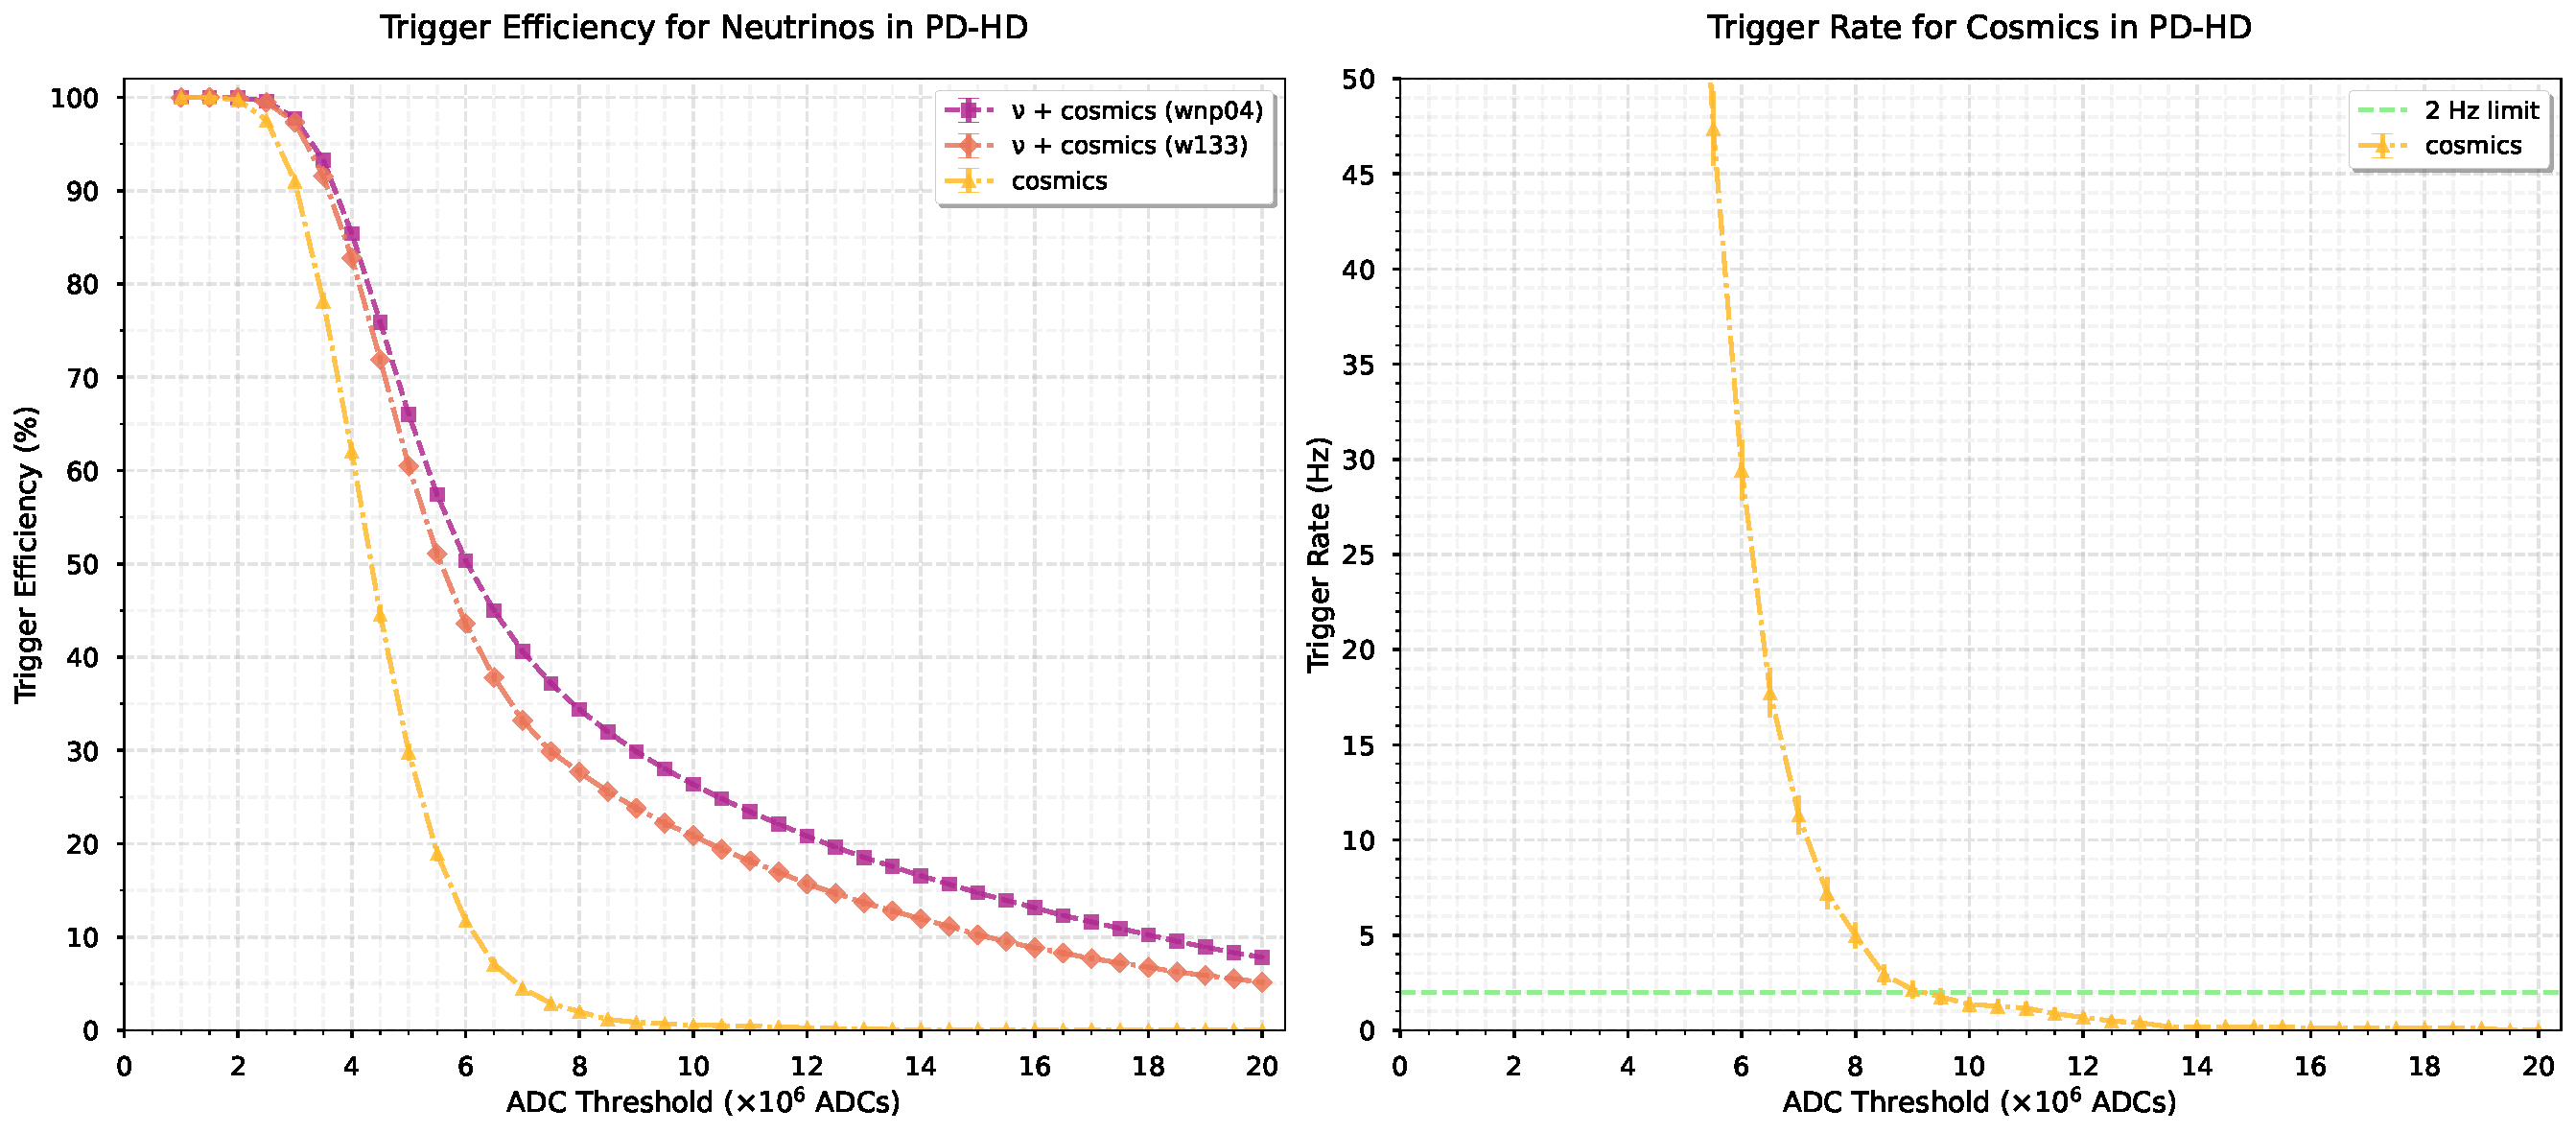
\includegraphics[width=\textwidth]{sections/trigger/plots/trigger_efficiency_and_rate_nu_NP04.pdf}
    \caption{Trigger efficiency for detected neutrinos, overlaid with cosmic-ray events, in PD-HD for wNP04 and w133 magnet configurations. The cosmic background trigger efficiency and rate are also present. The ADC threshold ranges from (0.5 to 20) million ADCs, and the time window is fixed to 0.32 ms.}
    \label{fig:trigger_performance}
\end{figure}

Figure \ref{fig:MC_trigger_efficiency} illustrates the simulated trigger performance for neutrinos interacting in ProtoDUNE over 1 week of SPS exposure for different magnet configurations. The orange histogram represents the energy distribution for all neutrinos interacting in the active TPC, while the blue histogram corresponds to those satisfying the trigger condition. The algorithm focuses on high-energy neutrinos to minimize the cosmic background and maintain a stable trigger rate of 1-2 Hz, as previously discussed.

\begin{figure}[]
	\centering
    \begin{subfigure}{0.65\textwidth}
	   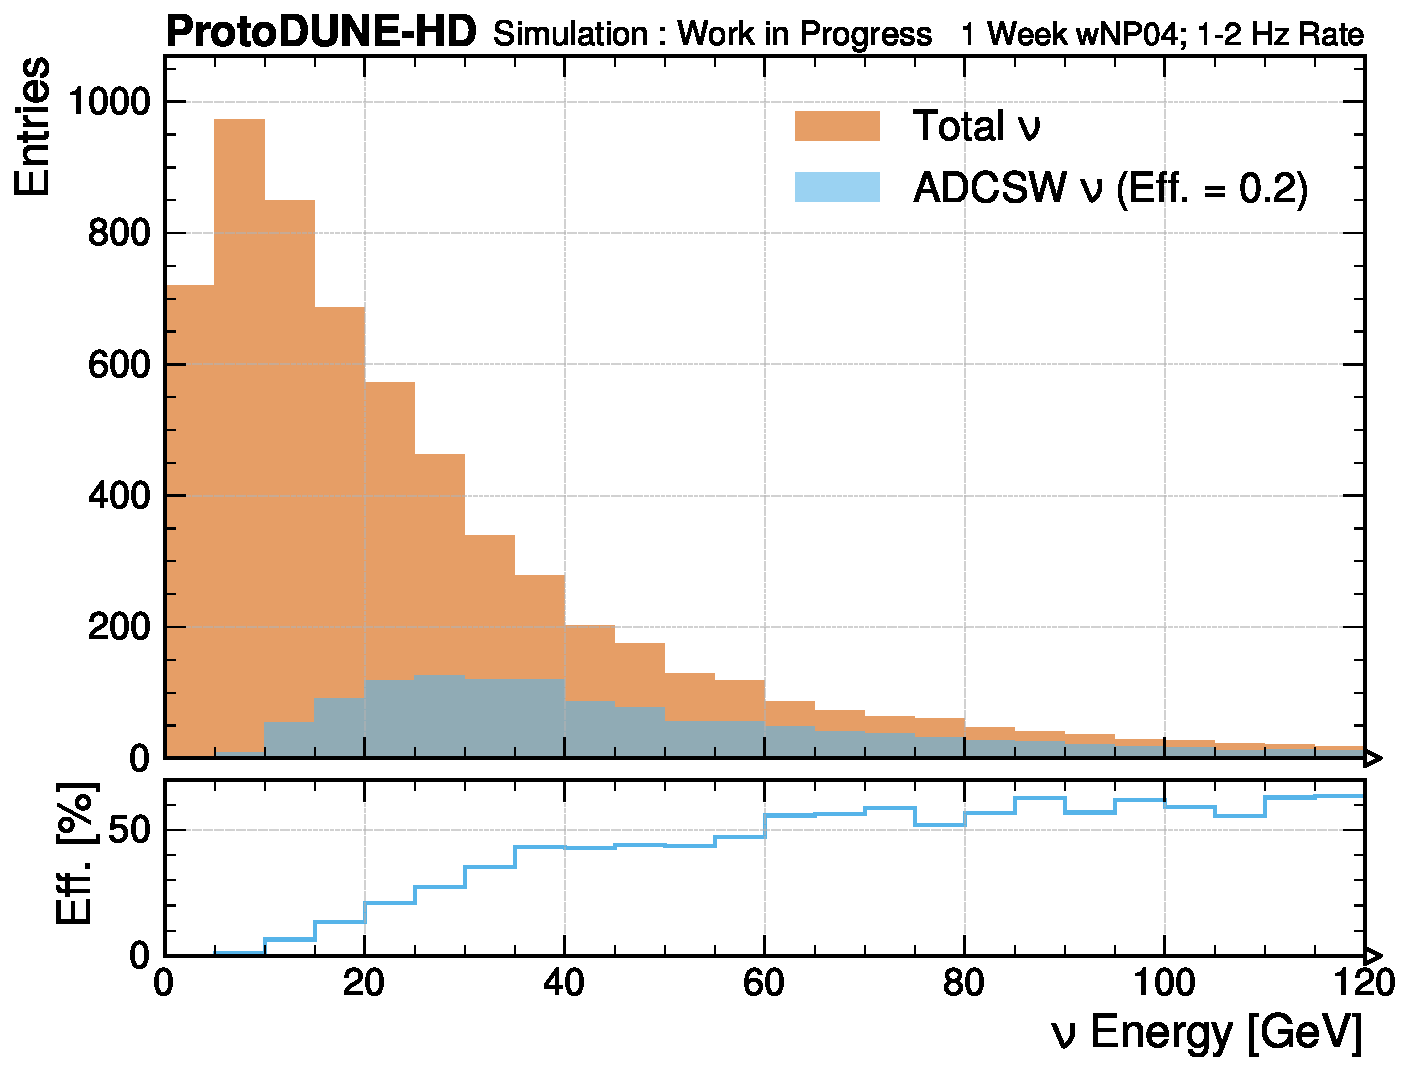
\includegraphics[width=0.99\columnwidth]{sections/trigger/plots/np04_wnp04_newlabel_adcsimplewindow_performance_nuE_1Hzrate_efficiency.pdf}
	   \caption{}
	   \label{fig:gifpp_triggerrate}
    \end{subfigure}

    \centering
    \begin{subfigure}{0.65\textwidth}
	   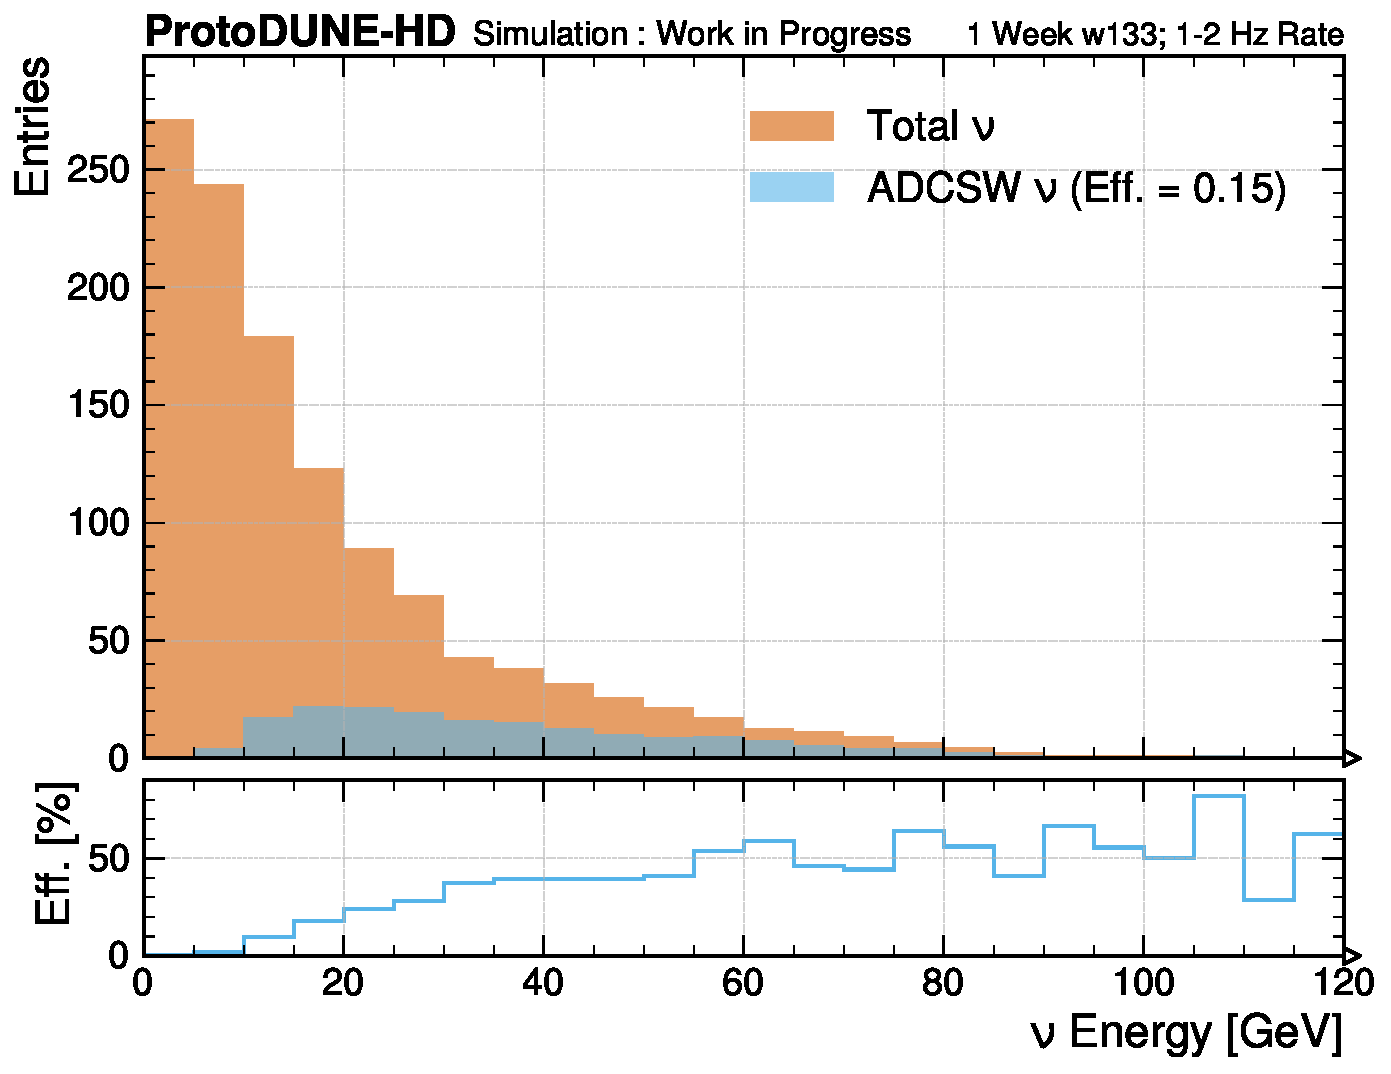
\includegraphics[width=0.99\columnwidth]{sections/trigger/plots/np04_w133_adcsimplewindow_performance_nuE_1Hzrate_efficiency.pdf}
	   \caption{}
	   \label{fig:w133_triggerrate}
    \end{subfigure}
    \caption{Figures~\ref{fig:gifpp_triggerrate} and \ref{fig:w133_triggerrate} show the trigger rate for neutrinos interacting during a wNP04 and w133 magnet configuration respectively. In both figures the orange histogram shows the total number of neutrinos interacting in PD-HD during one-week of SPS beam, whilst the blue histogram shows the number of neutrinos passing the trigger algorithm. The total trigger efficiency is indicated in the figure legends and the efficiency as a function of neutrino energy is plotted below each figure. The algorithm accounts for a time window length of 0.32 ms and an ADC threshold of $12 \times 10^6$ to effectively mitigate the cosmic background.}
    \label{fig:MC_trigger_efficiency}
\end{figure}

Since the TP generation was uniquely feasible at the collection plane of every APA, the trigger algorithm was using only that view, running simultaneously on each APA, and not including the induction planes. In contrast, raw waveforms were generated on each readout plane. It is noteworthy that the second induction plane for the APA1 functioned as the collection plane due to an inadequate bias voltage connection to the actual collection plane. Furthermore, ground shake events — spurious events with high saturation attributed to a sudden variation of the detector ground — were observed during data taking, as represented in Figure \ref{fig:ground_shake}. The ground-shake events are successfully filtered offline.
%Their origin still remains enigmatic. This feature has not compromised the data quality and only affects a small portion of the data. Overall, these events are completely vetoed by the DAQ system utilizing the above-mentioned algorithm, yet with a different parametrization according to the ground shake features. Only the first two runs (refer to table \ref{tab:data_table} in section \ref{chap:datasets}) present ground shake signals, with a custom labeled associated with the dedicated trigger, for further filtering in the LArSoft reconstruction chain.

\begin{figure}[h]
    \centering
    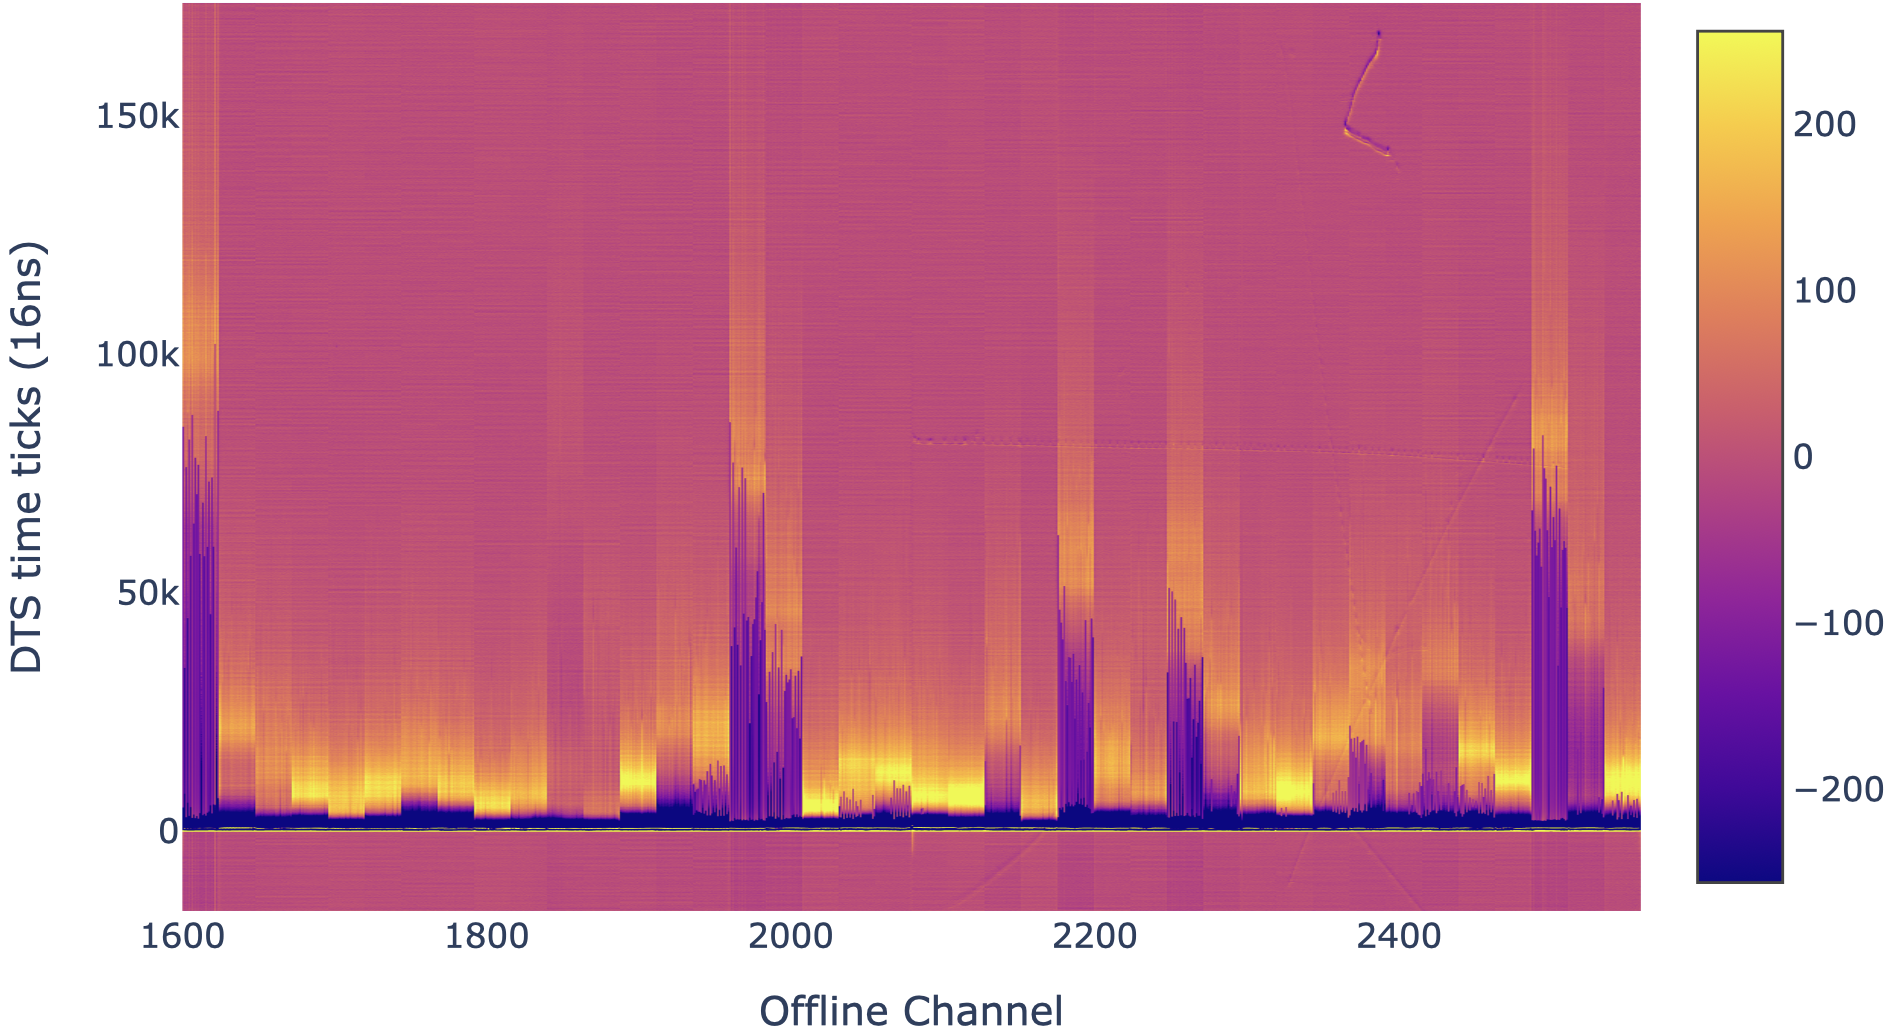
\includegraphics[width=0.8\linewidth]{sections/trigger/plots/ground_shake.png}
    \caption{Event display of a ground shake event in PD-HD during data taking. The distinct high saturation is correlated with a sudden variation of the detector ground. As per the ADC map, a complete channel multiplicity is also observed in the APAs.}
    \label{fig:ground_shake}
\end{figure}

%Since no particle beam is actually reaching PD-HD, the DUNE-DAQ system was unable to synchronize with the spill information. Consequently, data collection was conducted continuously, irrespective of the accelerator’s duty cycle: the trigger records events even when there are no protons on target capable of producing neutrino events. By filtering the events based on the spill flag, one can effectively eliminate a substantial number of cosmic events, allowing for an efficient selection of the potential sought-after signal events, which are inherently generated by the SPS accelerator and the T2 target. 
The data was collected continuously and the information between the TPC and the accelerator was correlated offline. In the analysis, the events are filtered based on the spill information, which reduces significantly the cosmic-ray induced events. 